\section{Creation of a Rydberg augmented basis set}
\label{sec:rydberg_procedure}

As already anticipated briefly, a Rydberg state is a particular kind of
electronically excited state where the electron is promoted into a
spatially diffuse orbital.  Given its high distance from the remaining
molecular electronic system, the spatial ``Rydberg'' orbital describing the
excited electron resembles an atomic orbital, where the ionized molecule is
seen as a positive pointcharge.  Almost all the structural differences are
lost due to distance, therefore slight changes in geometry does not affect
the Rydberg orbitals description.  For these reasons, the naming convention
for Rydberg orbitals resembles the one used for atomic orbitals, starting at
quantic number 3: Rydberg orbitals are named $3s$, $3p$, $3d$ and so on.
Also, it must be noted that the promoted electron has a very low correlation
with the remaining valence electrons.

Description of Rydberg states is complex: a Rydberg orbital is not
localized on an atom of the molecule, but on the molecule as a whole.
Standard basis sets are not able to correctly describe Rydberg orbitals,
therefore an enrichment with diffuse functions is needed to address these
cases. Two strategies exist for this task
\begin{itemize}
\item use an atom-centered basis set with both low-diffusion functions for the
description of the valence and high-diffusion functions for the Rydberg
orbitals. Linear combinations emerging from this basis set are able to describe
both types of valence and diffuse orbitals, left size of Fig.~\ref{fig:rydberg}
\item a standard basis set is used for the molecule, and a dummy X atom is added
holding a diffuse basis, right side of Fig.~\ref{fig:rydberg}
\end{itemize}

The first solution is simpler to use, but it produces a high number of not
interesting combinations. For the description of the 3s Rydberg, for
example, an ``all positive'' linear combination is needed, but this approach
also produces $p$, $d$, $f$... functions, arising from other combinations with
different sign. These combinations increase the computational cost and
introduce problems in the interpretation of data. 

The second technique reduces both problems, at the cost of introducing
complexity in the creation of the enriched basis set. In the subsequent
works, the second strategy has been used.

\begin{center}
\begin{figure}[ht]
\begin{center}
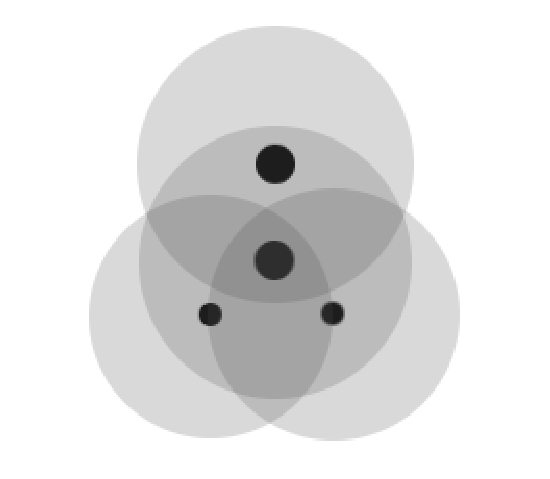
\includegraphics[width=5cm]{03_nevpt/images/rydberg1.eps}
\includegraphics[width=5cm]{03_nevpt/images/rydberg2.eps}
\end{center}
\caption{\footnotesize Two possible schemes to define an augmented basis set
for the description of diffuse Rydberg orbitals: adding diffuse functions on
the single atoms (left side of the picture) or adding diffuse functions
supported by a single dummy atom with no charge. In this thesis, the
development of the Rydberg orbitals followed the second approach.}
\label{fig:rydberg}
\end{figure}
\end{center}


\subsection*{Position of the charge centroid}

The position of the X dummy atom is usually chosen to coincide with the position of
the positive charge centroid, which depends on the molecular geometry and
the excitation performed. Various strategies could be devised in the
evaluation of these coordinates, but practical evaluations performed on
test molecules confirmed the very reduced dependency of the absolute energy
with respect to the dummy atom position. A possible strategy is represented 
by the procedure described by Roos and coworkers\cite{roos-qmescca}.

%A possible strategy is to devise an approximate position by means of the
%dipole $\mu$. For example, in the case of formaldehyde, the higher occupied
%orbitals (by symmetry) for the neutral system are $5a_{1},1b_{1},2b_{2}$.
%The standard geometrical orientation is assumed: the molecule is on the $zy$
%plane, with the carbonyl group along the $z$ axis.  To evaluate the Rydberg
%orbitals for an electronic transition of the type $n_{y} \rightarrow
%\mbox{Ryd}$, an electron is removed from $2b_{2}$. Using the program \dalton
%, a $B_2$ doublet can be evaluated with the following input
%\begin{verbatim}
%**DALTON INPUT
%.RUN WAVE FUNCTION
%.RUN PROPERTIES
%**WAVE FUNCTIONS
%.HF
%*HF INPUT
%.HF OCC
%5 1 1 0
%.MAX DIIS ITERATIONS
%50
%.OPEN SHELL
%3
%**PROPERTIES
%.POPANA
%*END OF INPUT
%\end{verbatim}
%A position for the centroid of the total positive charge can be evaluated
%using the formula
%\beq
%\overrightarrow{R}_{+} = \frac{\sum_{i} e_{+}(i) \overrightarrow{r}_{\! \! +}(i)}{\sum_{i} e_{+}(i)}
%\eeq
%where $i$ runs over the atoms, and $e_{+}(i)$, $\overrightarrow{r}_{\! \! +}(i)$ are
%the nuclear charge and the position of the atom $i$, respectively.
%The same relation could be written for the total negative charge centroid,
%making use of the Mulliken charges
%\beq
%\overrightarrow{R}_{-} = \frac{\sum_{i} e_{-}(i) \overrightarrow{r}_{-}(i)}{\sum_{i} e_{-}(i)}
%\eeq
%but a more accurate value can be obtained using the dipole as provided by \dalton
%\beq
%\overrightarrow{\mu} = \sum_{i} e_{+}(i) \overrightarrow{R}_{+} - \sum_{i} e_{-}(i)
%\overrightarrow{R}_{-}
%\eeq
%Finally, we can obtain the net charge centroid for the ionized molecule
%\beq
%\overrightarrow{R} = \frac{\sum_{i} e_{+}(i) \overrightarrow{R}_{+} + \sum_{i} e_{-}(i)
%\overrightarrow{R}_{-}}{\sum_{i} e_{+}(i) - \sum_{i} e_{-}(i) }
%\eeq
%where the X dummy atom will be placed. 

Another possible strategy is to choose the center of mass. This approach is
simpler, introducing a negligible change in the results, and removes the
need to evaluate the molecular dipole. In the evaluations performed later in
this thesis both approaches have been used, however as already stated
the choice of the position does not produce sizable effects on
the final result.

Once placed, the dummy X atom is provided with an uncontracted basis set.
The exponents for the gaussian functions can be obtained through a
universal algorithm by Kaufmann {\textit et al}\cite{jpb-22-2223-1989}.
\dalton provides an interface to generate these coefficients by means of the
\texttt{.CM FUN} keyword.  The keyword must be provided with three
numbers as defined in Ref. \citen{jpb-22-2223-1989}: the first number
indicates the maximal L quantum number desired for the generated functions.

The second number is related to the starting value for the exponents. The
chosen value gives exponents compatible with small molecules, such as
formaldehyde or acetone.  Kaufmann suggests using a value which provides
exponents in smooth continuity with the core basis set. 

The last number must be equal to or greater than the second, and produces a
new gaussian coefficient for every increment of $\frac{1}{2}$. 

In the performed evaluations the choice (2 2 5.5) has been made.
The first value 2 will generate $s$, $p$ and $d$-type Rydberg diffuse
functions, and the remaining two values 2 and 5.5 produce eight functions.
The final basis set on the X dummy atom is therefore the uncontracted
$8s8p8d$.  Exponents can be extracted from the output file of the \dalton
run.

\subsection*{Contraction of the Rydberg basis set}

The previous section demonstrated how to produce an uncontracted basis set
of diffuse gaussians. These gaussians can be used as-is to enrich the valence
basis set, providing a high number of degrees of freedom in the description of
high-energy Rydberg orbitals, but the resulting basis set is heavily
extended. This introduces a high computational cost and, in the case of
CASPT2 evaluations, convergence problems due to intruder states. 

For these reasons, it is often useful to contract the Rydberg basis set with
appropriate coefficients. A contraction from $8s8p8d$ to $1s1p1d$, for
example, leads to a reduction of the number of additional function from 72
to 9.  A more flexible choice is the contraction to $3s3p3d$, which gives a
good compromise between degrees of freedom and basis set reduction.

An explorative study has been performed to evaluate the influence of Rydberg
contraction on the energy of valence and Rydberg states of formaldehyde.
Tab.~\ref{tbl:rydberg_contraction} reports an evaluation performed on
various excited valence and Rydberg states of the formaldehyde. Details of
the evaluation will be presented in the next section, the only difference
being the basis set, in this case cc-pVTZ\cite{jcp-90-1007-1989}.

As can be seen, the reported values do not change significantly by
decontracting the Rydberg basis set. We can therefore conclude that a
contraction from $8s8p8d$ to $1s1p1d$ is mostly sufficient for obtaining
valuable results.

The procedure to obtain the contraction coefficients has been implemented
\textit{via} both \molcas and \texttt{DALTON}. The \molcas suite provides the \texttt{GENANO}
program, while for the \dalton program an analogous program
\texttt{GENANODAL} has been implemented by our research group.

\begin{center}
\begin{threeparttable}
\footnotesize
\begin{tabular*}{0.70\textwidth}{l@{\hspace{30mm}}cccc}
\hline
                       &  1 Ryd        &  3 Ryd        &  8 Ryd         \\
\hline
                        \multicolumn{4}{c}{\small A$_1$} 	\\
$n_y\!\!\rightarrow\!\! 3p_y$       &   8.14       & 8.14          &  8.14  \\
$n_y\!\!\rightarrow\!\! 3d_{yz}$    &   9.29       & 9.30          &  9.30 \\
$\pi\!\!\rightarrow\!\!\pi^{*}$     &   9.98       & 9.86          &  9.86 \\
                        \multicolumn{4}{c}{\small A$_2$} 	\\
$n_y\!\!\rightarrow\!\!\pi^*$       &   4.05       & 4.03          &  4.04 \\
$n_y\!\!\rightarrow\!\! 3p_x$       &   8.47       & 8.48          &  8.49 \\
$n_y\!\!\rightarrow\!\! 3d_{xz}$    &   9.47       & 9.50          &  9.50 \\
                        \multicolumn{4}{c}{\small B$_2$} 	\\
$n_y\!\!\rightarrow\!\! 3s$               &   7.38       & 7.38          &  7.38 \\
$n_y\!\!\rightarrow\!\! 3p_z$             &   8.29       & 8.24          &  8.24 \\
$n_y\!\!\rightarrow\!\! 3d_{x^2\!-\!y^2}$ &   9.26       & 9.22          &  9.22 \\
$n_y\!\!\rightarrow\!\! 3d_{z^2}$         &   9.43       & 9.39          &  9.39 \\
                        \multicolumn{4}{c}{\small B$_1$} 	\\
$n_y\!\!\rightarrow\!\! 3d_{xy}$          &   9.38       & 9.40          &  9.40 \\
$\sigma\!\!\rightarrow\!\!\pi^{*}$           &   9.37       & 9.33          &  9.33 \\
\hline
\end{tabular*}
\caption{\footnotesize An evaluation of valence and Rydberg excited states transition
energies of formaldehyde, using the cc-pVTZ basis set and different diffuse
basis set contractions. It can be noted that the contraction $8s8p8d$ to
$1s1p1d$ (1 Ryd) produces stable results.\label{tbl:rydberg_contraction}}
\end{threeparttable}
\end{center}


%The theoretical approach is rather simple: a matrix representation of the
%one-particle density matrix must be expressed in the atomic basis set. This
%can be obtained by expressing the one-particle density matrix on a basis set
%of generic spinorbitals $\left\{ \psi_i \left(i\right) \right\}$:
%\beq
%\rho\left(x, x^{\prime}\right) = \sum_{i,j} R_{i,j} \psi_{i} \left( i
%\right) \psi_{j}^{*} \left( x^{\prime} \right)
%\eeq
%Two particular choices of spinorbitals can be defined: the set $\left\{
%\phi_i \left(i\right) \right\}$ of pseudonatural orbitals of a given
%wavefunction and the set of functions used as the atomic basis set $\left\{
%\chi_i \left(i\right) \right\}$. Each one gives the one-particle
%density matrix through a different $R$ matrix
%\beqa
%\rho\left(x, x^{\prime}\right) &=& \sum_{i,j} R^{\mbox{NO}}_{i,j} \phi_{i} \left( i
%\right) \phi_{j}^{*} \left( x^{\prime} \right) \\
%&=& \mathbf{\phi} \mathbf{R}^{NO} \mathbf{\phi} \\
%\rho\left(x, x^{\prime}\right) &=& \sum_{i,j} R^{\mbox{AO}}_{i,j} \chi_{i} \left( i
%\right) \chi_{j}^{*} \left( x^{\prime} \right) \\
%&=& \mathbf{\chi} \mathbf{R}^{AO} \mathbf{\chi} 
%\eeqa
%A matrix of coefficients $\mathbf{C}$ expresses the combination of
%$\mathbf{\chi}$ to obtain $\mathbf{\phi}$
%\beq
%\mathbf{\phi} = \mathbf{\chi} \mathbf{C}
%\eeq
%the $\mathbf{\chi}$ basis set is not orthonormal, since
%\beq
%\mathbf{\chi}^{+}\mathbf{\chi} = \mathbf{S}
%\eeq
%Finally, $\mathbf{R}^{NO}$ is diagonal (given the definition) with
%occupation numbers on the diagonal. In general, the representation
%$R^{\mbox{AO}}$ is not diagonal. The following relation holds:
%\beq
%C^{-1}R^{AO}\left( C^{-1} \right)^{+} = R^{NO}
%\eeq
%Given the following 
%\beq
%\left( C^{-1} \right)^{+} = \left( C^{+} \right)^{-1} = SC
%\eeq
%we obtain
%\beq
%SR^{AO}SC = SCR^{NO}
%\eeq
%Where we obtain the coefficients and eigenvalues of $SR^{AO}S$ in
%a non-unity metric $S$. Once diagonalized, values for the X dummy atom are
%extracted, and a spherical normalization is performed for functions with
%symmetry different from $s$.

\subsection*{Using Molcas}

The procedure using the \molcas suite can be found in the manual
\cite{molcas-site}, and is also reported by Roos et al.\cite{roos-qmescca}.
Here a brief discussion will be presented. The needed steps are:
\begin{itemize}
\item add the diffuse, uncontracted basis set to the molecule (modifying the
\texttt{Seward} input file). The contraction coefficients matrix in this case is a
unit matrix
\item perform a CASSCF evaluation for the system with one electron removed
\item in the resulting output, identify the Rydberg orbitals described by one or
(probably) more functions on the X dummy atom
\item modify the \texttt{.RasOrb} file, containing the orbital coefficients
and their occupation numbers, setting the core occupation numbers to
zero. For the Rydberg orbitals, their occupation numbers must be set
to small, non-zero values, decreasing of one order of magnitude inside each
symmetry. The usual choice is 0.1, 0.01, 0.001 and so on. This prevents
mixing of different Rydberg orbitals inside the same symmetry
\item run the program \texttt{GENANO} with the modified \texttt{RasOrb}
file. This will produce contraction coefficients
\item finally, replace the contraction matrix into the \texttt{Seward} input
file with the new coefficients
\end{itemize}

\subsection*{Using Dalton}

The \dalton suite of programs does not implement a strategy for the
generation of contracted basis sets, therefore an external program has been
developed, named \texttt{GENANODAL}, to accomplish this task. The strategy
is as follows: 
\begin{itemize}
\item perform a Hartree-Fock open shell evaluation for the molecular ion
\item use the program \texttt{IJKLDALI} to perform orbital and integral reordering
\item run the program \texttt{GENANODAL} with an appropriate input, built using the
informations provided by \texttt{IJKLDALI}
\end{itemize}

An example input file is provided:
\begin{verbatim}
&LEGGI FILE11='/scr1/stef/$NAME/FILE11',
       FILE25='/scr1/stef/$NAME/FILE25',
  ZANO=T,NOCCUP=8*0.0,
  0.1,0.01,0.001,0.0001,45*0.0,
  0.0,0.1,0.01,21*0.0,
  0.1,0.01,24*0.0,
  0.1,
  NAOX=72,
  IAOX=23,24,25,26,27,28,29,30,
  64,65,66,67,68,69,70,71,
  92,93,94,95,96,97,98,99,
  31,32,33,34,35,36,37,38,
  39,41,43,45,47,49,51,53,
  40,42,44,46,48,50,52,54,
  72,73,74,75,76,77,78,79,
  100,101,102,103,104,105,106,107,
  111,112,113,114,115,116,117,118,
  MAXL=2,NPRIML=8,8,8,NANOL=1,2,3, &END
\end{verbatim}

\texttt{NOCCUP} have to be set to dummy occupation numbers for each orbital,
honoring the reordering performed by \texttt{IJKLDALI}. As in the case of
\texttt{MOLCAS}, these numbers must be set to values in descending order for the
Rydberg orbitals of the shell we are interested in.

\texttt{NAOX} and \texttt{IAOX} represent how many and which atomic
functions belong to the X dummy atom, repectively. These values must be
extracted from the \texttt{IJKLDALI} output.  The ordering of the functions
must be kept into account: first $s$-type functions, then $p$-type
functions, finally $d$-type functions.

\texttt{MAXL} is the maximal quantum number L to extract. In this case, up to $d$-type
functions are requested.

\texttt{NPRIML} is the number of primitives for each quantum number. For contracting
a $8s8p8d$ Rydberg basis, these values are 8,8,8.

Finally, \texttt{NANOL} are the number of contracted functions generated for each
quantum number L. In this case, provided only as an example, 1 $s$-type
contracted function will be produced, along with 2 $p$-type functions and 3
$d$-type functions. From the output, only the first column of coefficients
will be used.

The \texttt{GENANODAL} code provides exactly the same results as obtained from the
\molcas chain.
